\pagebreak
\onecolumn
\begin{center}
    \Large
    \textit{Generalized Perturbations} Scenario
\end{center}

All the plot included here are available as interactive html (for proper 3D visualization and zooming) at \url{https://fraiori0.github.io/antip-handover/}, along with videos of the interactions.

\begin{figure*}[h!]
    \centering
    \subfloat[\footnotesize Interaction A.1. The participant takes back the hand after reaching out (as described in Sec. \ref{sec:introduction}), before reaching again for the handover. \label{fig:perturbed:B.2}]{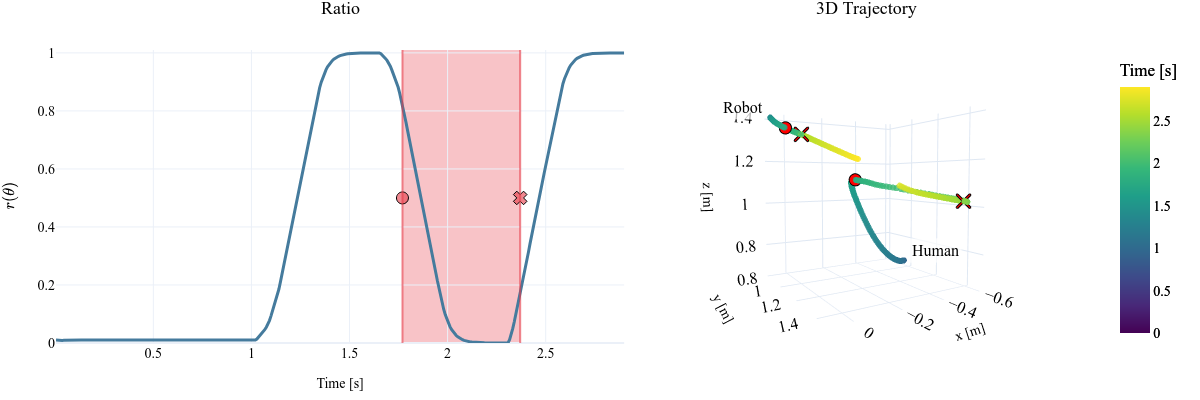
\includegraphics[width=0.65\textwidth]{figs/perturbed_ratio_3d/A.1.png}}
    \\
    \subfloat[\footnotesize Interaction A.2. The participant takes back the hand after reaching out (as described in Sec. \ref{sec:introduction}), before reaching again for the handover. \label{fig:perturbed:B.2}]{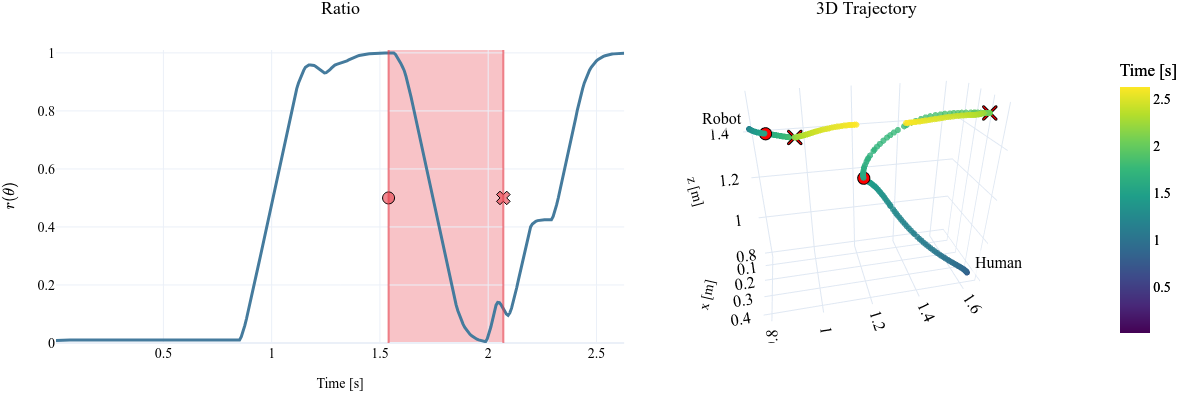
\includegraphics[width=0.65\textwidth]{figs/perturbed_ratio_3d/A.2.png}}
    \\
    \subfloat[\footnotesize Interaction B.1. The participant waves their hand before reaching for the handover. \label{fig:perturbed:B.2}]{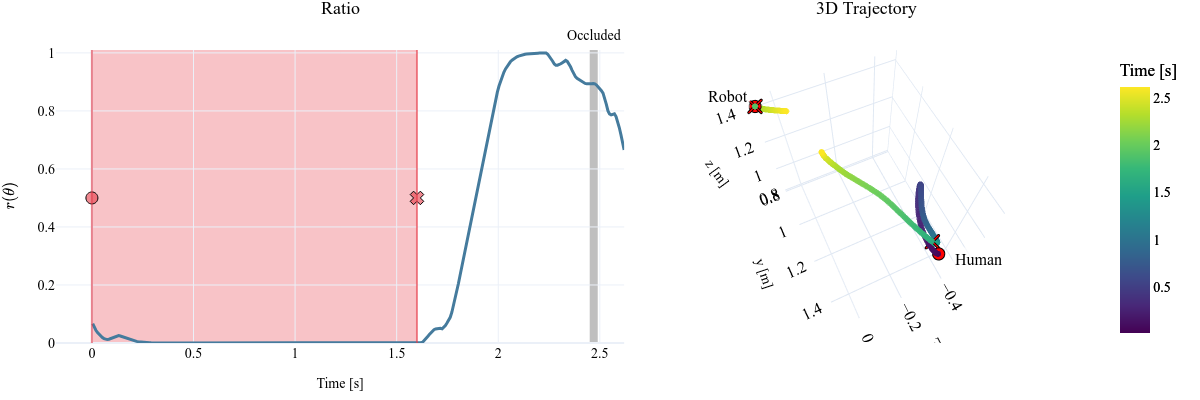
\includegraphics[width=0.65\textwidth]{figs/perturbed_ratio_3d/B.1.png}}
    \\
    \subfloat[\footnotesize Interaction B.2. The participant waves their hand before reaching for the handover. \label{fig:perturbed:B.2}]{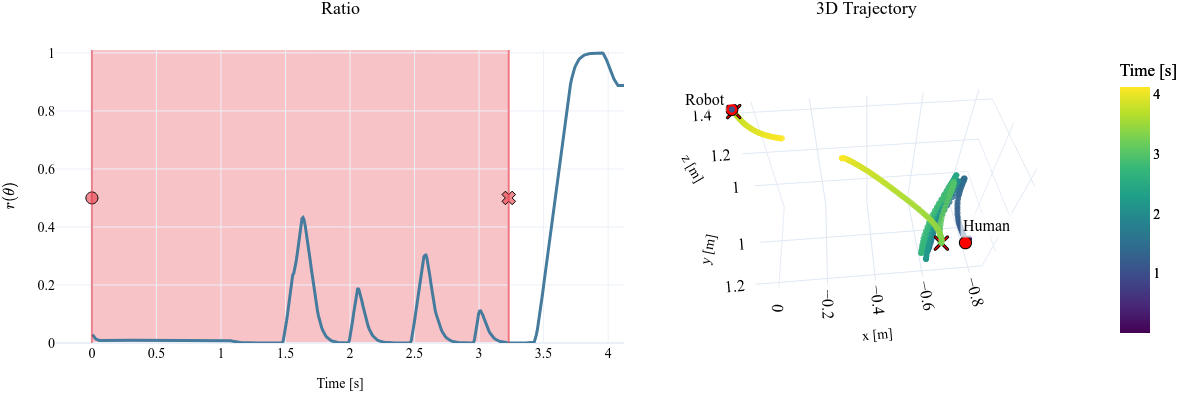
\includegraphics[width=0.65\textwidth]{figs/perturbed_ratio_3d/B.2.png}}
    \hfill
    \caption{Evolution of the ratio and 3D trajectory of interactions A and B in the General Perturbation scenario.
    The red shaded area denotes the time between the start and the end of the perturbation.
    The red circle and cross show the points selected as the start and the end of the perturbation, respectively.
    The color scale denotes corresponding time steps in the two trajectories, with points recorded at the same time as the same color.
    Finally, the gray shaded area denotes part of the interaction where the human hand was occluded; the 3D plot shows a hypothetical interpolated trajectory with small pink markers.
    }
    \label{fig:perturbed:A_B}
\end{figure*}


\begin{figure*}[h!]
    \centering
    \subfloat[\footnotesize Interaction C.1. The participant's hand is slapped. \label{fig:perturbed:2}]{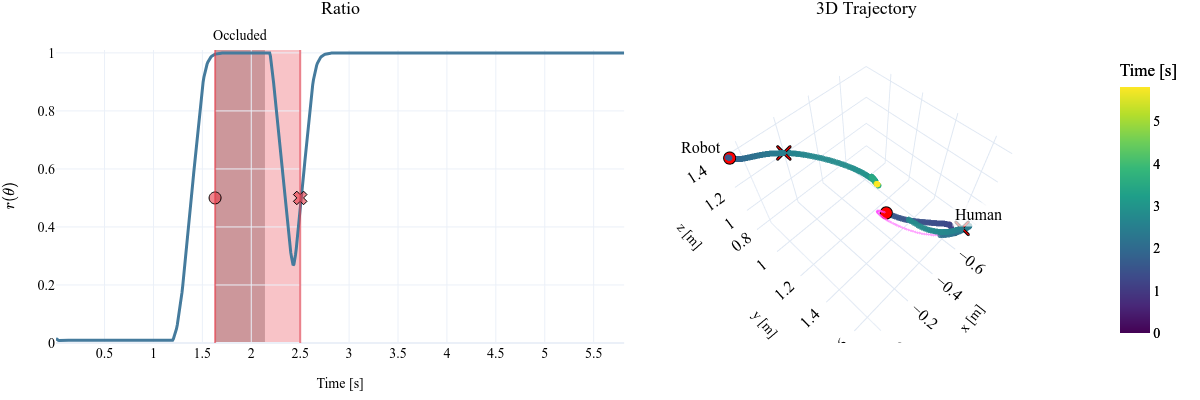
\includegraphics[width=0.65\textwidth]{figs/perturbed_ratio_3d/C.1.png}}
    \\
    \subfloat[\footnotesize Interaction C.2. The participant's hand is slapped. \label{fig:perturbed:2}]{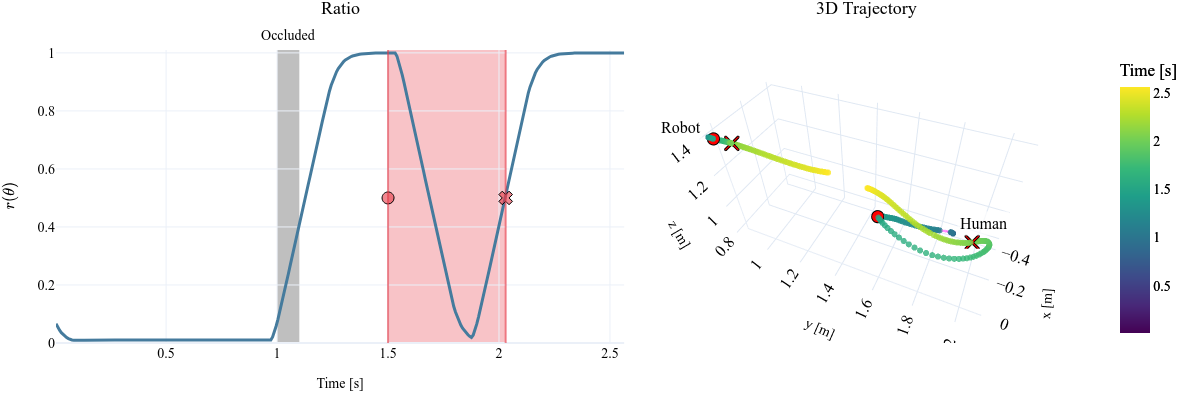
\includegraphics[width=0.65\textwidth]{figs/perturbed_ratio_3d/C.2.png}}
    \\
    \subfloat[\footnotesize Interaction D.1. The participant is thrown a light plastic toy. \label{fig:perturbed:3}]{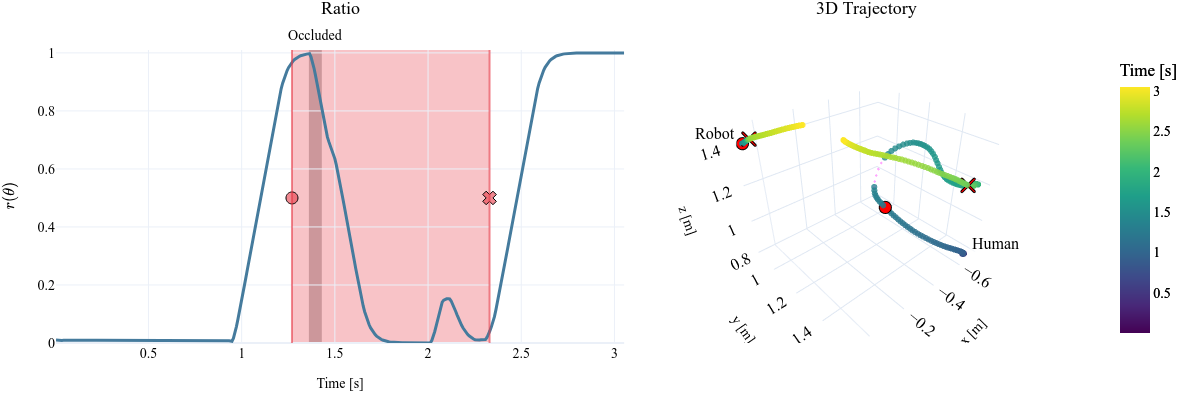
\includegraphics[width=0.65\textwidth]{figs/perturbed_ratio_3d/D.1.png}}
    \\
    \subfloat[\footnotesize Interaction D.2. The participant is thrown a light plastic toy. \label{fig:perturbed:3}]{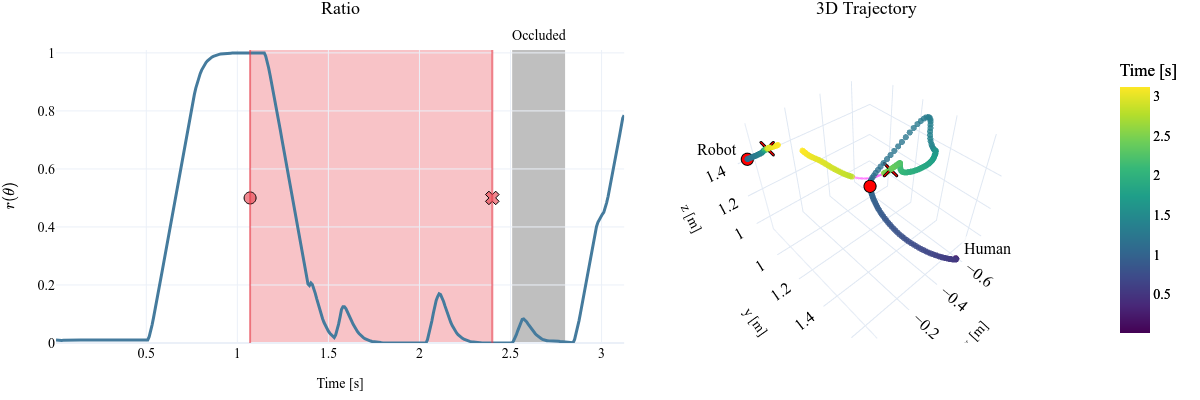
\includegraphics[width=0.65\textwidth]{figs/perturbed_ratio_3d/D.2.png}}
    \hfill
    \caption{Evolution of the ratio and 3D trajectory of interactions C and D in the General Perturbation scenario.
    The red shaded area denotes the time between the start and the end of the perturbation.
    The red circle and cross show the points selected as the start and the end of the perturbation, respectively.
    The color scale denotes corresponding time steps in the two trajectories, with points recorded at the same time as the same color.
    Finally, the gray shaded area denotes part of the interaction where the human hand was occluded; the 3D plot shows a hypothetical interpolated trajectory with small pink markers.
    }
    \label{fig:perturbed:C_D}
\end{figure*}

\begin{figure*}[h!]
    \centering
    \subfloat[\footnotesize Interaction E.1. The participant is thrown a basketball. \label{fig:perturbed:2}]{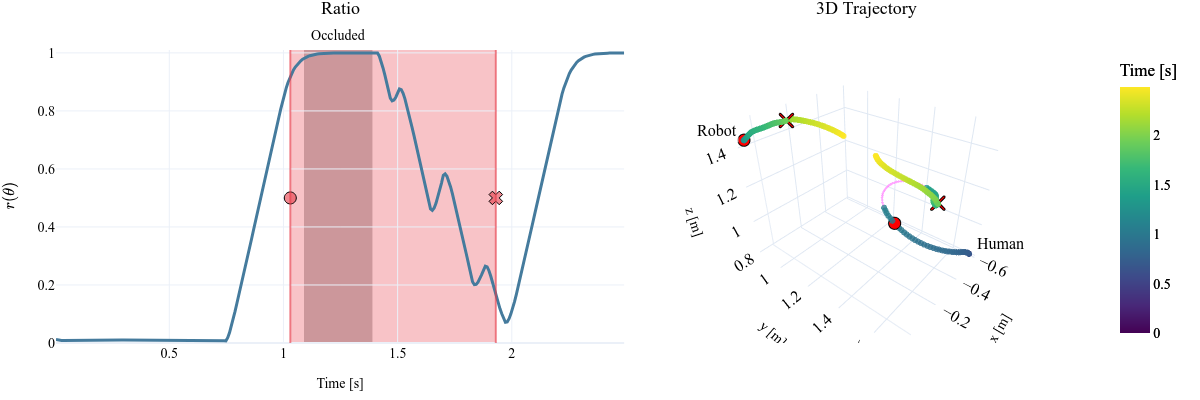
\includegraphics[width=0.65\textwidth]{figs/perturbed_ratio_3d/E.1.png}}
    \\
    \subfloat[\footnotesize Interaction E.2. The participant is thrown a basketball. \label{fig:perturbed:2}]{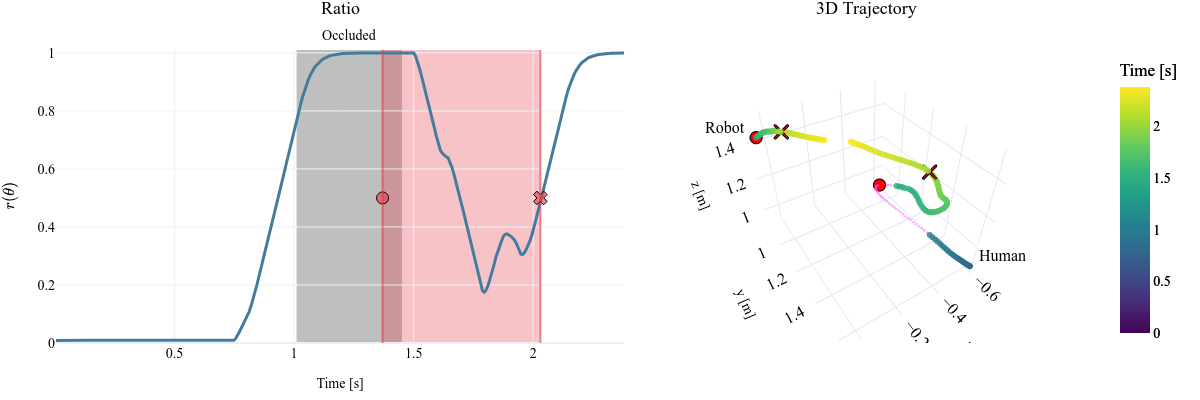
\includegraphics[width=0.65\textwidth]{figs/perturbed_ratio_3d/E.2.png}}
    \\
    \subfloat[\footnotesize Interaction F.1. The participant is thrown a large beanbag. \label{fig:perturbed:3}]{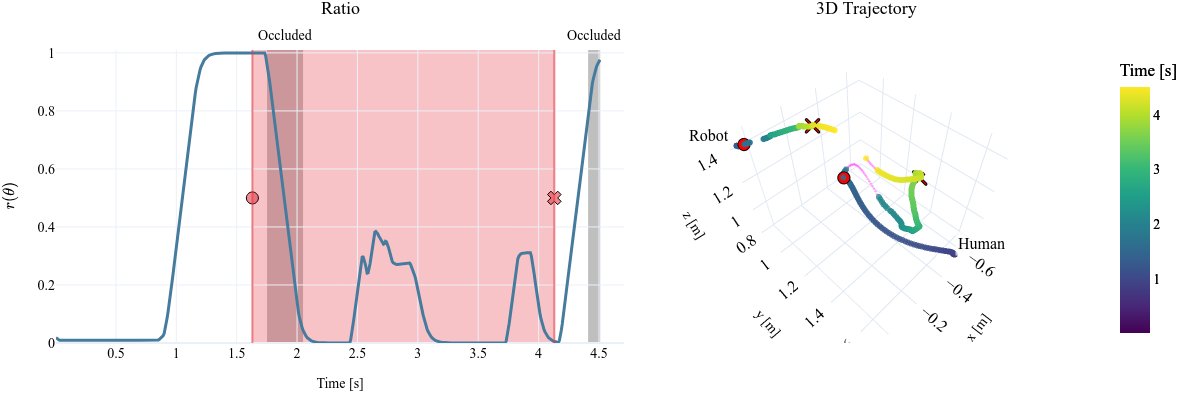
\includegraphics[width=0.65\textwidth]{figs/perturbed_ratio_3d/F.1.png}}
    \\
    \subfloat[\footnotesize Interaction F.2. The participant is thrown a large beanbag. \label{fig:perturbed:3}]{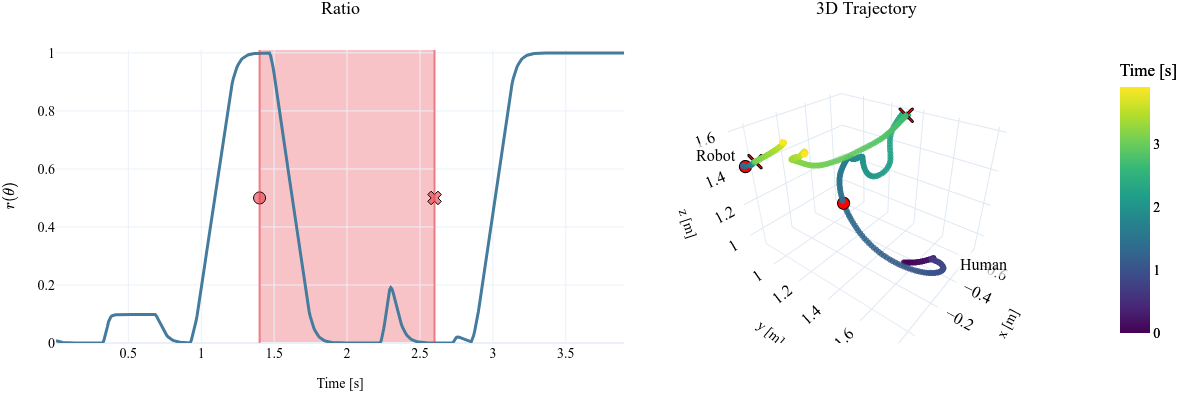
\includegraphics[width=0.65\textwidth]{figs/perturbed_ratio_3d/F.2.png}}
    \hfill
    \caption{Evolution of the ratio and 3D trajectory of interactions E and F in the General Perturbation scenario.
    The red shaded area denotes the time between the start and the end of the perturbation.
    The red circle and cross show the points selected as the start and the end of the perturbation, respectively.
    The color scale denotes corresponding time steps in the two trajectories, with points recorded at the same time as the same color.
    Finally, the gray shaded area denotes part of the interaction where the human hand was occluded; the 3D plot shows a hypothetical interpolated trajectory with small pink markers.
    }
    \label{fig:perturbed:E_F}
\end{figure*}